\section*{Formalism}
    \subsection{Mathematical context}
        The system evolve on a field which should be mapped with the magnetometer. It follows the evolution describe by \textsc{Equation}~\ref{eqn:state_eqn}.
        \begin{equation}
            \label{eqn:state_eqn}
            \begin{cases}
                \dot{\mathbf{x}} = f(\mathbf{x}(t), \mathbf{u}(t)) &(evolution\ equation)\\
                \mathbf{y}^i = g(\mathbf{x}(t_i)) &(observation\ equation)
            \end{cases}
        \end{equation}

        where $\mathbf{x}$ is the state of the robot, $\mathbf{u}$ is the input of the system. As $\mathbf{x}$ and $\mathbf{u}$ continuously evolve with time, we define the trajectories of this system denoted by $\mathbf{x}(\cdot)$ and $\mathbf{u}(\cdot)$. We could also define tubes enclosing these trajectories at every time denoted by $\forall t, [\mathbf{x}](t)$ and $\forall t, [\mathbf{u}](t)$. Measurements are available at each $t_i$ and are denoted by $\mathbf{y}^i$. Therefore it is assumed that $\forall t, \mathbf{u}(t) \in [\mathbf{u}](t)$ and that for each measurements $\mathbf{y}^i \in [\mathbf{y}^i]$. This last conditions means that each measurement is bounded which is an assumption made frequently when we are dealing with constrain programming.

    \subsection{State equations}
        The system is composed of a vehicle that will drag a sledge that transports a magnetometer. The towing vehicle is a tank type vehicle, and the sled is attached to it with a rope. Assuming that the rope is constantly under tension, we are able to find the equations describing the dynamics of the system.
        \begin{subequations}
            \begin{empheq}[left={f(\mathbf{x}(t), \mathbf{u}(t))=\empheqlbrace}]{align}
                \dot{\mathbf{x}}_1 & = \tfrac{\mathbf{u}_1 + \mathbf{u}_2}{2}.cos(\mathbf{x}_3) \\
                \dot{\mathbf{x}}_2 & = \tfrac{\mathbf{u}_1 + \mathbf{u}_2}{2}.sin(\mathbf{x}_3) \\
                \dot{\mathbf{x}}_3 & = \mathbf{u}_2-\mathbf{u}_1 \\
                \dot{\mathbf{x}}_4 & = -\tfrac{\mathbf{u}_1 + \mathbf{u}_2}{2}.sin(\mathbf{x}_4) - \dot{\mathbf{x}}_3
              \end{empheq}
        \end{subequations}

        Here $\mathbf{x}_1$, $\mathbf{x}_2$ and $\mathbf{x}_3$ are respectively the abscissa, the ordinate and the heading of the trailing robot, $\mathbf{x}_4$ is the angle of the sled to the tractor vehicle, as shown in \textsc{Figure}~\ref{fig:state_variables}. We can also notice that $\tfrac{\mathbf{u}_1 + \mathbf{u}_2}{2}$ is related to the speed control of the char robot and that $\mathbf{u}_2-\mathbf{u}_1$ is the angular acceleration control.

        \begin{figure}[!htb]
            \centering
            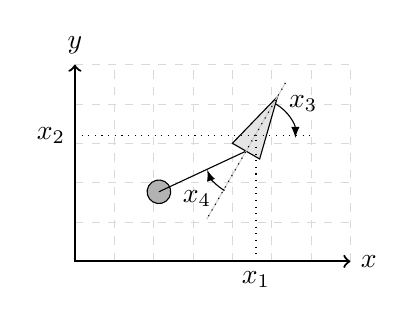
\begin{tikzpicture}
                \draw[help lines, color=gray!30, dashed, step=0.5] (0,0) grid (3.5,2.5);
                \draw [<->,thick] (0,2.5) node (yaxis) [above] {$y$}
                    |- (3.5,0) node (xaxis) [right] {$x$};

                \tikzset{
                    robot/.pic = {
                        \draw[black,fill=gray!20] (0,0) -- (0.2,0.8) -- (0.4,0) -- cycle;
                        \draw[black,fill=gray!60] (0.2,0) -- (-0.5,-1) circle(0.15);
                        \draw[gray!40] (0.2,-1) -- (0.2,1);
                        \draw[dotted] (0.2,1) -- (0.2,-1);

                    }
                }
                \pic[rotate=-30] at (2, 1.5) {robot};
                \draw[dotted] (0,1.6) node (x2) [left] {$x_2$} -- (2.3,1.6) -- (2.3,0) node (x1) [below] {$x_1$};
                
                \draw[dotted] (2.3,1.6) -- (3,1.6);
                \draw[>=latex, ->] (2.55,2) arc (60:0:0.5);
                \draw node at (2.9,2) {$x_3$};
                \draw[>=latex, ->] (1.9,0.9) arc (240:200:0.5);
                \draw node at (1.55,0.8) {$x_4$};
            \end{tikzpicture}
            \caption{Diagram representing system state variables}
            \label{fig:state_variables}
        \end{figure}
